\chapter{Predefined Knowledge Ports}
Knowledge ports are building blocks of Shark based applications.
Each Shark project will create its own knowledge port. Some are
already shipped with the framework. Number of such ready-to-use
ports will increase with each new version. The first and most flexible 
implementation is the {\tt StandardKP} though. 

\section{StandardKP}
\label{sec:knowledgePorts:StandardKP}
The  {\it Shark basic scenario} was explained in section \ref{sec:concepts:baseScenario}: Alice and Bob met. Both are interested in {\it P2P system}. Both found out their mutual interest by means of interest exchange and ultimately, knowledge was transfered.

{\tt StandardKP} was developed to serve such scenarios. This section reveals how this basic scenario can be implemented with a few lines of code.

But let's start from the beginning: {\tt StandardKP} extends {\tt KnowledgePort}. It isn't abstract and implements {\tt doExpose()} and {\tt doInsert()} it triggers {\tt KPListener} objects.

Each {\tt StandardKP} must be instantiated with an interest and a knowledge base. This KP can actually be seen as the guard that serves as an extractor and
assimilator of knowledge. The interest can be seen as a filter for both exporting and importing. 

We are going to finish the introduction and start with the program. Actually, we are going two write two programs: One plays the role of Alice, the other the role of Bob. Source code can also be found on sharksystem.net under tutorials.

The following section will contain the complete Alice program and the section after will cover Bob's point of view. Relevant algorithms are explained afterwards.

\subsection{Alice and Bob basic scenario}
\subsubsection{Alice}
\begin{verbatim}
public class Alice implements KPListener {
  public static SharkEngine aliceSE;

  public static void main(String[] args) throws ... {
    // Create a new SharkEngine
    aliceSE = new J2SEAndroidSharkEngine();

    // Create a new knowledge base for this Alice
    SharkKB kb = new InMemoSharkKB();

    // Create a peer to describe the topic "Shark"
    SemanticTag shark = kb.createSemanticTag
                           ("Shark",
                            "http://www.sharksystem.net/");
    
    // Create a peer semantic tag describing Alice herself
    String[] aliceAddr = new String[1];
    aliceAddr[0] = "tcp://localhost:7070";
 
    PeerSemanticTag alice = aliceKB.createPeerSemanticTag(
                              "Alice", 
                              "http://www.sharksystem.net/alice.html", 
                              aliceAddr);

    // Alice owns this SharkKB
    aliceKB.setOwner(alice);

    // Create new coordinates before creating a ContextPoint
    ContextCoordinates cc = aliceKB.createContextCoordinates(
                              sharkST, /* topic */
                              alice, /* originator */
                              alice, /* peer */ 
                              null, /* remote peer: any*/ 
                              null,  /* time: any */
                              null, /* place: any */
                              SharkCS.DIRECTION_OUT);

    // Create a ContextPoint to add information to
    ContextPoint cp = aliceKB.createContextPoint(cc);
 
    // Add a string to the ContextPoint at the given coordinates
    cp.addInformation("I like Shark");

    // Create a StandardKP with engine, kb and interest
    StandardKP kp = new StandardKP(aliceSE, cc, aliceKB);
 
    // set up listener
    Alice alicePeer = new Alice();
    kp.addListener(alicePeer);
 
    // Start listening at TCP port 7070
    aliceSE.startTCP(7070);

    // Now the peer is passively waiting for incoming traffic

    // Create description if Bob
    PeerSemanticTag bob = aliceKB.createPeerSemanticTag(
                            "Bob", 
                            "http://www.sharksystem.net/bob.html", 
                            "tcp://localhost:7071");

    // publish interest to start communication
    // assumes that bobPeer is already up and running
    aliceSE.publishKP(kp, bob);
  } // end main methods

  /* KPListener implementation */
  public void exposeSent(KnowledgePort kp, 
                         SharkCS sentMutualInterest) {
    // ignore
  }

  public void insertSent(KnowledgePort kp, 
                         Knowledge sentKnowledge) {
    // Alice shuts down after sending knowledge
    System.out.println(
       "Alice has sent something - enough for today...");
    aliceSE.stop();
  }

  public void knowledgeAssimilated(KnowledgePort kp, 
                                   ContextPoint newCP) {
    // ignore
  }
} //end Alice class
\end{verbatim}

Only fourteen lines of code are required to write a P2P program that does a useful job. Additional lines are required to implement the {\tt KPListener}. We had some larger programs when we explained knowledge extraction etc. The reason for this is that {\tt StandardKP} perfoms the complete communication between knowledge base and external peer(s). 

Let's investigate the program. Most of it was explained in previous chapter. We create a {\tt SharkEngine} which makes up the peer. We have created a {\tt SharkKB} which holds semantic tags and information.

A semantic tag is created that describes {\it Shark}. A peer semantic tag is created describing Alice herself. In this example, she has just a single address: A TCP port at local host. That's not advisable for real applications but its a good decision testing.

{\tt ContextCoordindates} are created. They use {\it Alice} as originator and peer and {\it Shark} as topic. Information shall be sent which is defined by 
{\tt DIRECTION\_OUT}. A context point is created and a brief information added.

Neither of those lines are new. New is creation of the {\tt StandardKP} with three parameters: the {\tt SharkEngine}, the {\tt interest} (we re-use our coordinates) and the {\tt SharkKB}. That's it. Out {\tt StandardKP} has anything it needs: It knows what is Alice willing to talk about and it knows where to store and/or retrieve information.

A KPListener is set up afterwards - just to illustrate its usage.

\begin{verbatim}
aliceSE.startTCP(7070);
\end{verbatim}

This line tells the engine to open a TCP port and to accept incoming KEP messages. Now the Alice peer is ready to retrieve information. 

In this example, Alice initiates communication. A peer semantic tag is used to describe bob. His peer is listening at port 7071 on the same machine which will hardly be used in real applications but in tests.

\begin{verbatim}
aliceSE.publishKP(kp, bob);
\end{verbatim}

This line forces the engine to take the {\it interest} from the {\tt kp} and send it to {\tt Bob}. An {\it expose} message is sent from Alice to Bob. That's it. Communication has started.

The KPListener implementation is trivial. Alice peer stops communicating after sending a single knowledge object, see {\tt insertSent} implementation.

\subsubsection{Bob}
The following program implements Bob who is also interested in Shark. He wants just receive information but not send anything. The following lines are just the main method of the Bob peer.

\begin{verbatim}
// SharkEngine bobSE is declared as member variable
// create engine
bobSE = new J2SEAndroidSharkEngine();

// Create an in memory knowledgebase for information storage
SharkKB kb = new InMemoSharkKB();

// Describe Shark
SemanticTag shark = kb.createSemanticTag("SharkFW", 
                      "http://www.sharksystem.net/");

// Create a peer to describe ourselves (Bob)
String[] bobAddr = new String[1];
bobAddr[0] = "tcp://localhost:7071";

PeerSemanticTag bob = kb.createPeerSemanticTag("Bob", 
                        "http://www.sharksystem.net/bob.html", 
                        "tcp://localhost:7071");

// Create an interest 
ContextCoordinates interest = kb.createContextCoordinates(
    shark, /* topic */ 
    null, /* originator: any */
    bob, /* peer */,
    null, /* remote peer: any */ 
    null, /* time: any */
    null, /* location: any */ 
    SharkCS.DIRECTION_IN /* looking for information */
);

// Create Standard knowledge port
StandardKP kp = new StandardKP(bobSE, interest, kb);

// Start listening at TCP port 7071
bobSE.startTCP(7071);
\end{verbatim}

\subsection{doExpose}
Both program are quite short. That's because the application logic is hidden in the {\tt StandardKP}. We are going to describe the algorithm that is performed when an interest is received.

Figure \ref{fig:StandardKP_expose} summarizes the standard expose process.
Yes, that figure is confusing. We will go through it step by step.

Colors describe different types of aspects in that figure. Yellow is used to mark algorithms. Red is used to indicate member variables of the {\tt StandardKP}. All of them can be set either with a constructor or other methods.

Blue illustrates a process that issues a KEP message. There is a single green entity which is a message from a remote peer. Arcs describe the flow of control. Dashed arcs show what member variable is input for a process. Now we can start investigating the process.

\paragraph{Interest arrives}
The whole process is started whenever an {\it interest} was received. The {\tt SharkEngine} performs a preprocessing which is explained later in section {\ref{sec:sharkengine} in more details. Just in brief: Developers can define security policies and black- or white list. That means, developers can define if messages from other peers must be signed and/or encrypted or not. A white list contains all peers from which this peer is willing to accept messages at all. Developers can also decide to maintain a black list that contains peer from which no further messages are accepted.

Those checks are already made before a knowledge port starts working at all.
Thus, the interest that was received in the upper left corner is from an accepted peer and satisfies security settings of this peer.

\paragraph{Revealing check}
{\tt StandardKP} objects are created with an interest. We call it 
{\it local interest}. 
In most cases, a local interest contains semantic tag sets in its dimension. Alice in our example described her interest in {\it Shark} with a semantic tag in her topic dimension.

The received interest can contain semantic tags e.g. in its topic dimension. In this case, a later process figures out whether or not both topic sets match with each other. This process is described soon.

The received interest can also have an empty e.g. topic dimension. An empty dimension is interpreted as {\it anything}. Alice could receive such an interest. She would know, that this peer is apparently interested in anything. She could calculate that it is also interested in {\it Shark}.

Let's consider this step from a privacy point of view. Peers could send any interests to other peers. Those peers would reveal their interests as reply. There is a unbalanced situation in case of an {\it any interest}. The sending peer reveals nothing of its interest. Alice reveals her interest.

Developers can decide if this unbalanced situation is bearable or not. The {\tt setRevealLocalInterest(boolean)} methods can be used to define what policy shall be used. {\tt True} would allow revealing local interests even if the remote peer just send {\it any} tags. That's default behavior because in most cases peers should learn from each other at least vocabulary.

The default behavior can be switched off. In this case, the process is continued only if each non-any dimension of the local interests meets a non-any dimension in received interest.

\begin{figure}[t]
\centering
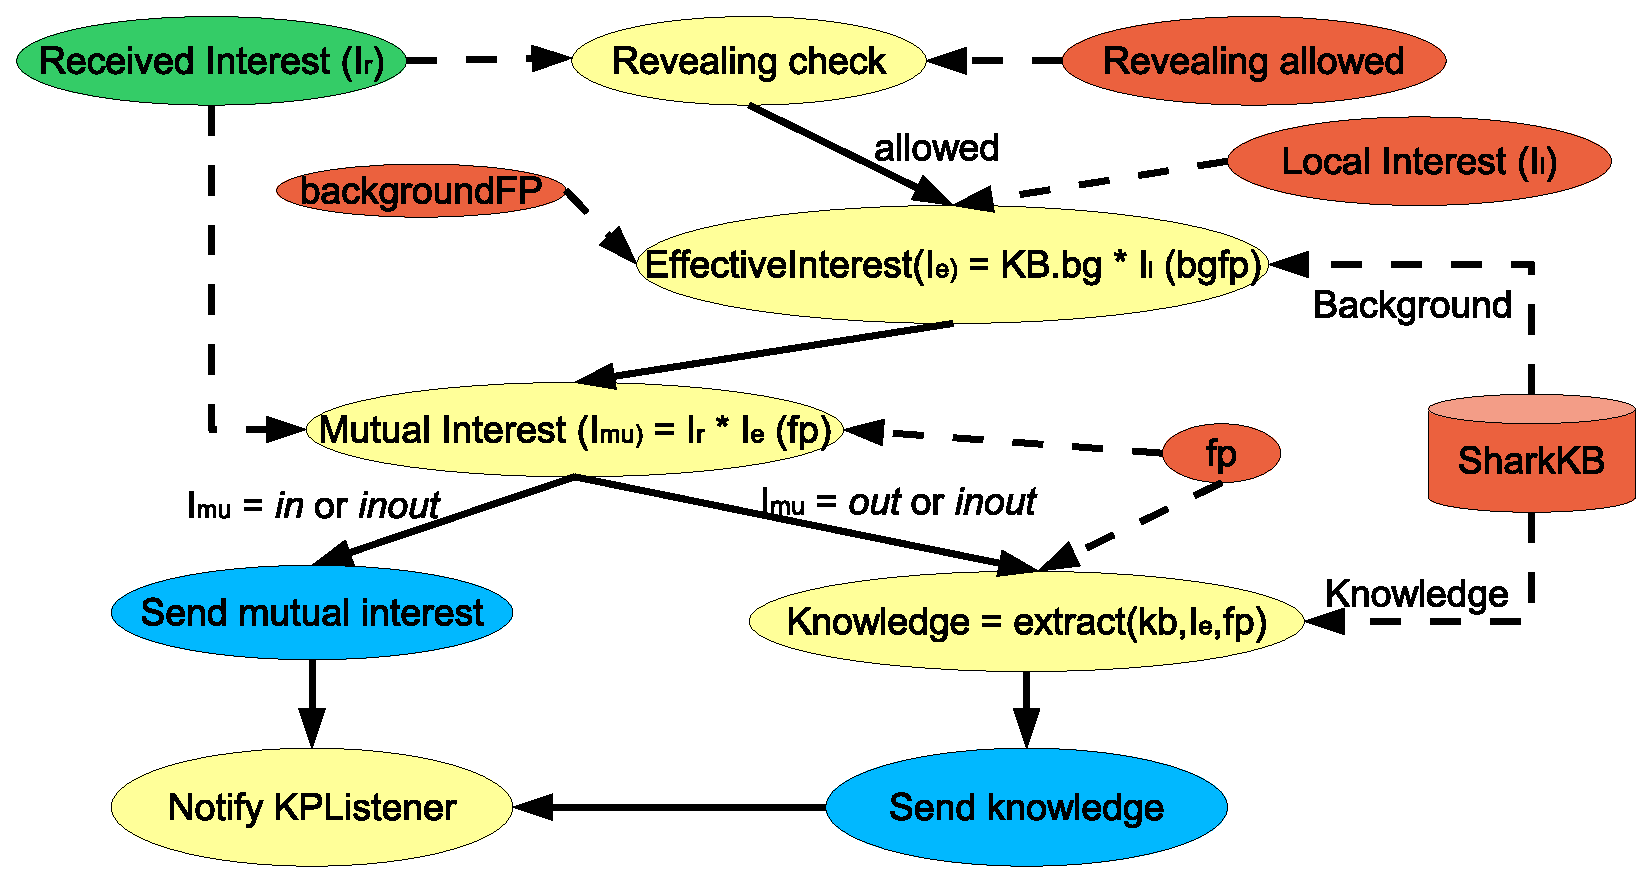
\includegraphics[width=1.00\textwidth]{StandardKP_Expose.eps}
\caption{StandardKP expose algorithm}
\label{fig:StandardKP_expose}
\end{figure}

\paragraph{Effective Interest}
Bob is the remote peer in our example and Alice receives his interest. {\tt StandardKP} calculates the {\it effective interest} by contextualizing the background knowledge with the local interest and some given fragmentation parameters (backgroundFP). What is that good for?

A knowledge base can change. Alice might decide to add information about a Shark application, e.g. {\it SharkNet}. {\it SharkNet} would be a semantic tag and would have a relation to {\it Shark}. Alice has already defined her local interest. She declared her interest to share information about {\it Shark}. What if she wants to share also information regarding SharkNet? 

Shark assumes that a local interest can be seen as an anchor. It assumes, that related information shall also be shared automatically to some degree.

The knowledge base background contains the up-to-date vocabulary of each peer. It is taken as source and contextualized with the local interest which serves as context in this case. The {\tt backgroundFP} parameter configures this process. Alice could e.g. define to share sub-topics of {\it Shark} but no super-topics. She could also declare to share nothing that the local interest by setting backgroundFP-{\tt depth} to zero in each dimension. 

The result of this calculation is called {\it effective interest}. It can be more general if {\tt backgroundFP} allows fragmentation in some degree. It can only be smaller if {\tt backgroundFP} is zero and tags used in local interest are removed from vocabulary.

Otherwise and in most cases, the {\it effective interest} is larger than or identical to the {\it local interest}.

\paragraph{Mutual Interest}
The received interest is taken and contextualized with the effective interest. Fragmentation parameter (fp) manages this process. This step less complicated than the others. A remote peer, e.g. Bob, showed its interest in communication. The local peer, Alice in this case, calculated her up-to-date interest.

Now she uses Bobs interest as source and finds out what of her interests fits to him. If Bob would be interested in {\it Sports} and she is interested in {\it Shark} no match can be found. If Bob is interested in {\it anything} {\it Shark} would be found as mutual interest, see discussion about revealing several lines above.

The result is called {\it mutual interest}. A mutual interest is assumed to be empty if at least a single dimension could not find a match, see also former section about contextualization of interests.

The process stops if no mutual interest can be found. No message is sent to the other peer. The algorithm is just finished.

\paragraph{Receiving Mutual Interest}
The mutual interest can be a receiving interest which means the direction is either {\tt IN} or {\tt INOUT}. In this case, the mutual interest is send back to the remote peer. Finally, the knowledge port listener are informed about that action.

\paragraph{Sending Mutual Interest}
The mutual interest can be a sending interest which means the direction is either {\tt OUT} or {\tt INOUT}. Knowledge is extracted from the local knowledge base with help of the effective (!) interest and the fragmentation parameter {\tt fp}. Extracted knowledge is sent to the remote peer. Listeners are informed about this action.

\subsubsection{In simple words...}
That was a big deal of details. Nevertheless it was necessary but now we can have a more abstract view on that algorithm. 

\begin{itemize}
\item 
A peer defines its interest by a {\it local interest}.
\item 
It also defines two fragmentation parameter, {\tt backgroundFP} and {\tt fp}. 

\item 
{\tt backgroundFP} is used to create an up-to-date interest. It take the local interest as anchor and finds related (and maybe new) tags in the vocabulary. This {\it effective interest} can change when peers vocabulary changes.

\item
Effective interest is used to calculate the {\it mutual interest} which comprises things that both peers share. Fragmenation parameter {\tt fp} is used here. It can be assumed that an empty mutual interest is quite common in most applications.

\item
Finally, the mutual interest itself is replied or knowledge that was extracted by means of the mutual interest. 
\end{itemize}

Developers should define interest very carefully. Developers can forbid revealing interest and set {\tt depth} to zero in {\tt backgroundFP} or even {\tt fp}. After getting used to those methods, both constraints can be relaxed. But start with the reduced view to be on the safe side. Open your system later step by step when you became familiar with it.

\subsection{constructor and parameters}
The previous process is quite complex. Handling received knowledge is easier. The good point is that we know all parameters which are used in {\tt StandardKP}. The most general constructor is this:

\begin{verbatim}
public StandardKP(SharkEngine se, SharkCS interest, 
   FragmentationParameter[] backgroundFP, 
   FragmentationParameter[] fp, SharkKB kb) {
\end{verbatim}

\begin{description}
\item[se] is an engine object. Each peer requires a single SharkEngine. It keep all components together. An engine must exist before creating a knowledge port. Engine are discussed in next chapter.

\item[interest] is an interest that defines constraints under which the peer is willing to exchange knowledge. 

\item[backgroundFP] is a fragmentation parameter. It is used to update the local interest. In general, it can enhance he rules under which a communication can take place. It takes out the up-to-date background from the knowledge base for this task. 

As broader it is defined as more learn peers from each other. Learning and spying are opposite sides of the same coin, though. Developers have to consider how to use it: Being more open, more verbose or more safe, less open. If you have doubts, use {\tt KnowledgePort.getZeroFP()}. It return is parameter that is set to depth 0 and doesn't allow following any relation to other tags in any dimension.

\item[fp] is also a fragmentation parameter. It is used to find mutual interests. Thus, is the parameter which configures how much information get into the knowledge base. {\tt BackgroundFP} configures how much knowledge leaves the peer.

\item[kb] is the a knowledge of this peer. {\tt StandardKP} can changes vocabulary and information depending on parameters and received messages.
\end{description}

There are two other constructor. Here is one:
\begin{verbatim}
public StandardKP(SharkEngine se, SharkCS interest, 
  FragmentationParameter[] fp, SharkKB kb) {
    this(se, interest, fp, fp, kb);
}
\end{verbatim}

This constructor can be used of both fragmentation parameters are identical, e.g. {\tt zeroFPs}.

Last one comes here.
\begin{verbatim}
public StandardKP(SharkEngine se, SharkCS interest, SharkKB kb) {
  this(se, interest, KnowledgePort.getZeroFP(), 
    KnowledgePort.getZeroFP(), kb);
}
\end{verbatim}

Both fragmentation parameters are set to zero. Changing vocabulary won't have any effect on communication behavior. It is the proposed constructor for beginners. It has no side effects which can arise from an growing vocabulary or added information.

\subsection{doInsert}
{\tt StandardKP} can also process incoming knowledge. The algorithm is less complex than the previous one. Figure \ref{fig:StandardKP_insert} illustrates the steps and used parameter.

\begin{figure}[t]
\centering
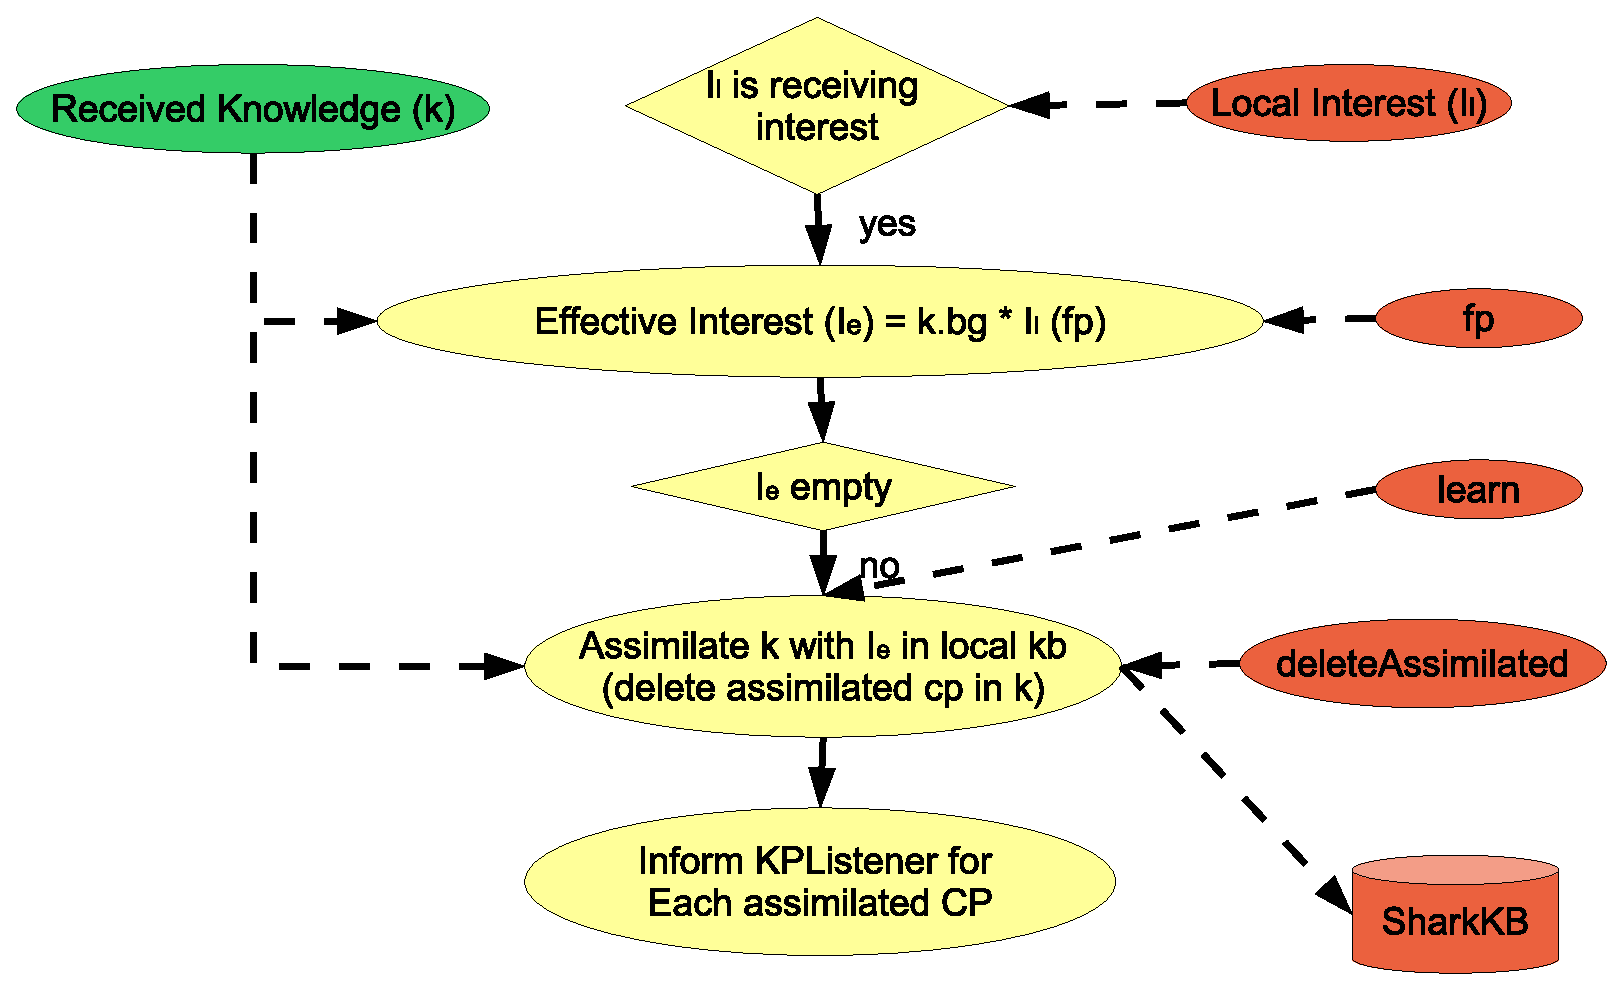
\includegraphics[width=1.00\textwidth]{StandardKP_Insert.eps}
\caption{StandardKP insert algorithm}
\label{fig:StandardKP_insert}
\end{figure}

First of all, it is checked whether the local interest is a receiving interest. More specific, it is checked if the direction is set to {\tt IN} or {\tt INOUT}. We also call such ports {\it IKP - incoming knowledge ports.}. Ports defining their direction with {\tt OUT} are called {\it OKP - outgoing knowledge ports}. A local interests with a direction setting of {\tt INOUT} is both IKP and OKP.
We need an IKP here because knowledge has arrived and there must at least the general interest in receiving something. 

Now, vocabulary (in other words:background knowledge) is taken and contextualized with the local interest by means of the fragmentation parameter. 
The result is an {effective interest}. It contains tags which are in the knowledge and which also fit to local interest. Thus, the receiving vocabulary is reduced in most cases to tags which fit to peers interests.

The process already ends if the {\it effective interest} is empty. An assimilation process is started otherwise. We have already discussed assimilation in a previous chapters. In short: Each context point is investigated. It is calculated if it fits into the context space defined by the {\it effective interest}. Thus, each, no or some context points can be added to the local knowledge base. 

{\tt StandardKP} allows learning of tags. Thus, peers vocabulary grows if context points are assimilated that have unknown tags which are related to known tags. This default behavior can be changed by {\tt learningSTs(false);} Vocabulary remains unchanged in the mode but coordinates of assimilated context points might change.

Assimilated context points are removed from the received knowledge in default. This has, of course, no effect on senders knowledge base. It has an effect on subsequent calls of other knowledge ports, though. They cannot assimilate the same context points again. This default behavior shouldn't be changed in applications with a single knowledge base. It is fully sufficient that one port adds a fitting context point the local knowledge base. Applications using more knowledge bases should consider to change that setting. The default behavior can be changed with {\tt deleteAssimilatedFromKnowledge(false)}.

\subsection{Summary}
{\tt StandardKP} is complex, no doubt about it. But it is complex inside. It can be used quite simple. Developers can start with the easiest constructor and use default settings. Peers will exchange knowledge and learn vocabulary from each other but with less surprises. Our Alice and Bob basic scenario hopefully helps.
It is simple and is neither long nor complex.

Once you have became familiar with it, start experimenting with those fragmentation parameters. It is not complicated but sometimes tricky.

\section{HubKP}
\label{sec:hubkp}
In social groups, a {\it hub} is a person that knows a noteworthy number of other people. A hub is a match maker. In Shark, a hub is a knowledge port that collects and delivers interests of others. 

\begin{figure}[t]
\centering
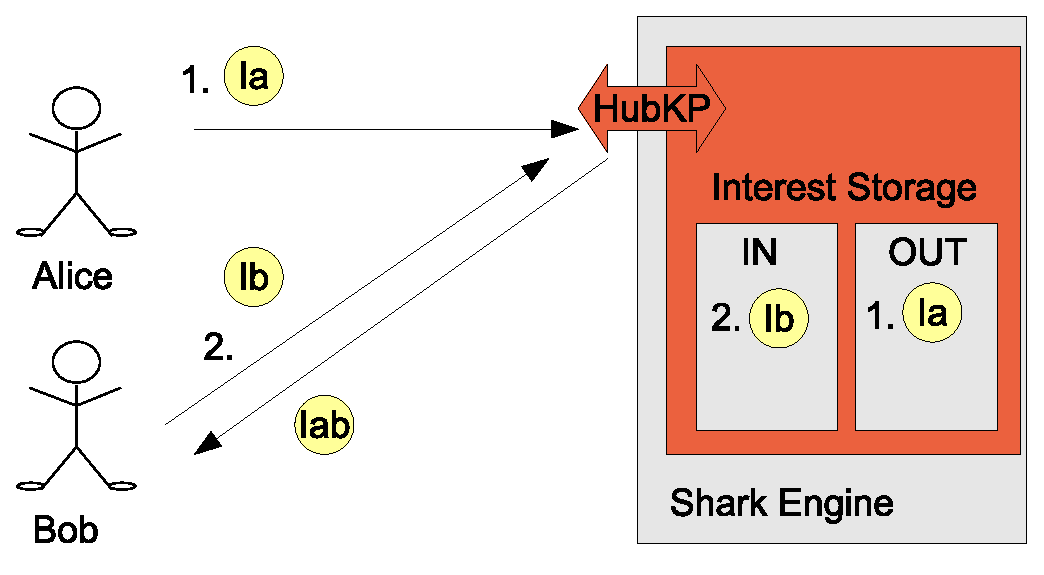
\includegraphics[width=0.70\textwidth]{hubKP.eps}
\caption{HubKP - general idea}
\label{fig:hubKP}
\end{figure}

Figure \ref{fig:hubKP} illustrates an example. There is a SharkEngine on the right. It can run e.g. on a mobile phone. That engine has a running {\tt HubKP} which has its own interest storage. Actually, that storage is separated into a receiving and sending interests. 

The little scenario starts with Alice. She is still and always interested in sending information. In our example, she is the first who communicates with that engine. Her interest arrives the engine and is offered to any active knowledge port. {\tt HubKP} becomes active. It hasn't met any other peer and its interest storage is empty. Thus, is just stores the interest and does not reply to Alice.

Bob arrives later and issues his interest. He is still interested in receiving information. The hub takes that interest and stores it as well. Then is calculates: Bob is interested in receiving something. Thus, hub checks its sending interest storage. It takes any interest and calculates the {\it mutual interest}. Non-empty mutual interest are send back as reply. Bob receives a mutual interest of his and Alice interest. 

The hub performs the same operation as Bob would do if he would have received that interest from Alice. Even the result is the same. Both mutual interests are identical. 

There are differences of course.

\begin{itemize}
\item 
A hub helps to bring peers together. Alice and Bob don't have to meet to learn about their mutual interests. Hub collects interests and makes those calculations for other peers.
\item 
Peers do not send all their interests to hubs - at least, they shouldn't. A hub runs a peer. Peers can always decide what to expose to whom. A trustworthy friend can know interests of personal matter. An anonymous peer shouldn't. 
Thus, when meeting an anonymous hub, peers would send only interests which can be published to literally anybody. 
\end{itemize}

That example is perfect to remember the difference between logical and physical sender. In this case, Bob gets a mutual interest. That interest contains a peer in the remote peer dimension. It is Alice. Alice issued her interest in the first place to the hub. Hub just stores the interest and calculates mutual interest after receiving an interest from Bob. The logical sender is Alice. She willingly (or not) stored her interest with the hub.

The physical sender is the hub, though. Thus, Bob can decide how to handle that result. In most cases, it would hurt to handle the result as trustworthy. In this case, Bob would expose a subsequent interest to directly to Alice if he could found her permanent address (e.g. mail address) in remote peer dimension. 

Alice would now receive an interest directly from Bob. A direct P2P communication is established now and End-to-End-Security could be established.

This book to teach programming with Shark. Therefore, we have a look into the implementation. Source code can be found in our open software repository. Visit our web page where to find our repository. (It was Projekt SharkFW on GitHub when this chapter was written).

\subsection{Usage}
Usage of the hub port is very simple. Once a {\tt HubKP} is instanciated on a {\tt SharkEngine} it offers hub features to other peers.

\begin{verbatim}
SharkEngine se = ... // was created earlier in code

KnowledgePort hub = new HubKP(se, 3600);
\end{verbatim}

Two features are to be noted:

\begin{enumerate}
\item 
This hub implementation has no persistent memory. All stored interest get lost if the port or the whole engine terminates. It's a feature. Hub is not (yet) intended to be a permanent kind of directory for peer interests.
\item 
Second parameter describes lifetime of interest in the hub storage. In this example, interest are forgotten after 3600 seconds which is one hour.
\end{enumerate}

\subsection{Implementation} 
We won't explain each line of code but the core parts of the class. Nevertheless, the whole implementation has 145 lines of code with comment lines. 
If you are curious - have a look into our source code repository.

{\tt HubKP} has to implement the {\tt doInsert} method. This method is abstract in class {\tt KnowledgePort} and {\tt HubKP} must have an implementation to become a non-abstract class. The implementation is empty, though:

\begin{verbatim}
@Override
protected void doInsert(Knowledge k, KEPConnection responseFactory) {
     // Do nothing. We don't process inserts.
}
\end{verbatim}

A hub does not deal with information but with interests. There is nothing to do for it when receiving information.

It implements {\tt doExpose}. The following code was copied from
the repository. Some unimportant lines and comments are removed to
spare space.

\begin{verbatim}
protected void doExpose(SharkCS interest, 
                        KEPConnection kepConnection) {
  try {
    // process interest
    if(interest.getDirection() == SharkCS.DIRECTION_IN || 
        interest.getDirection() == SharkCS.DIRECTION_INOUT) {

       this.doProcess(interest, kepConnection, this.outInterests);
   }

   if(interest.getDirection() == SharkCS.DIRECTION_OUT || 
       interest.getDirection() == SharkCS.DIRECTION_INOUT) {

       this.doProcess(interest, kepConnection, this.inInterests);
   }
  }
  catch(SharkException e) {
   L.l("failure while processing interest in HubKP.);
  }

  // finally save it
  if(interest.getDirection() == SharkCS.DIRECTION_IN || 
       interest.getDirection() == SharkCS.DIRECTION_INOUT) {
   
      this.inInterests.addInterest(interest);
  }

  if(interest.getDirection() == SharkCS.DIRECTION_OUT || 
       interest.getDirection() == SharkCS.DIRECTION_INOUT) {
   
      this.outInterests.addInterest(interest);
  }
}
\end{verbatim}

There are just two parts in method implementation. First, it is checked whether received interest is a receiving interest (direction is IN or INOUT) or a
sending interest (direction is OUT or INOUT). An interest with INOUT in its direction is both and is handled twice. 

The method doProcess is called with the received interest, {\tt kepConnection} and the appropriate interest storage. {\tt outInterests} contains received sending interests. They could match with an receiving interest and vice versa.

The second part stores received interest in its storage. Again, an INOUT interest is stored in both storages.

That's not really difficult. Neither is {\tt doProcess}:

\begin{verbatim}
private void doProcess(SharkCS interest, 
                       KEPConnection kepConnection, 
                       InterestStore storedInterests) 
                  throws SharkKBException, SharkException {

  Iterator<SharkCS> interestIter = storedInterests.getInterests();

  while(interestIter.hasNext()) {
      SharkCS storedInterest = interestIter.next();

      // mutual interest?
      Interest mutualInterest = SharkCSAlgebra.contextualize(
          storedInterest, interest, fps);

      if(mutualInterest != null) {
          kepConnection.expose(mutualInterest);
      }
  }
}
\end{verbatim}

{\tt doProcess} is called with the received interest and a storage of already stored interests which could fit. {\tt kepConnection} is required to reply.

First, an iterator is created that iterates any stored interests. Variable 
{\tt storedInterest} refers to an stored interest in each loop. A mutual interest is created for each combination (received and stored interest).
A non-empty mutual interest indicates both peers have something in common: The peer that was just met and the peer from which hub had stored its interest. 

The action is straightforward: A non-empty mutual interest is exposed to
the peer that issued its interest. In our previous example, the hub would find Alice interest in its storage and send Bob the non-empty mutual interest.

That's it. We won't discuss the interest storage implementation. It organizes removal of outdated interests. That's no rocket science. Have a look into the code.

We are ready with {\tt HubKP}. It isn't difficult, is it? Let's have a look on a sketch of a chat implementation with knowledge ports.

\section{ChatKP}
\label{sec:chatkp}
A chat is a pretty simple distributed system. A peer creates a message and wants it send to a recipient. Recipient shall read the message and can reply. This principle has to translated into the Shark concept. And this easy.

\begin{figure}[t]
\centering
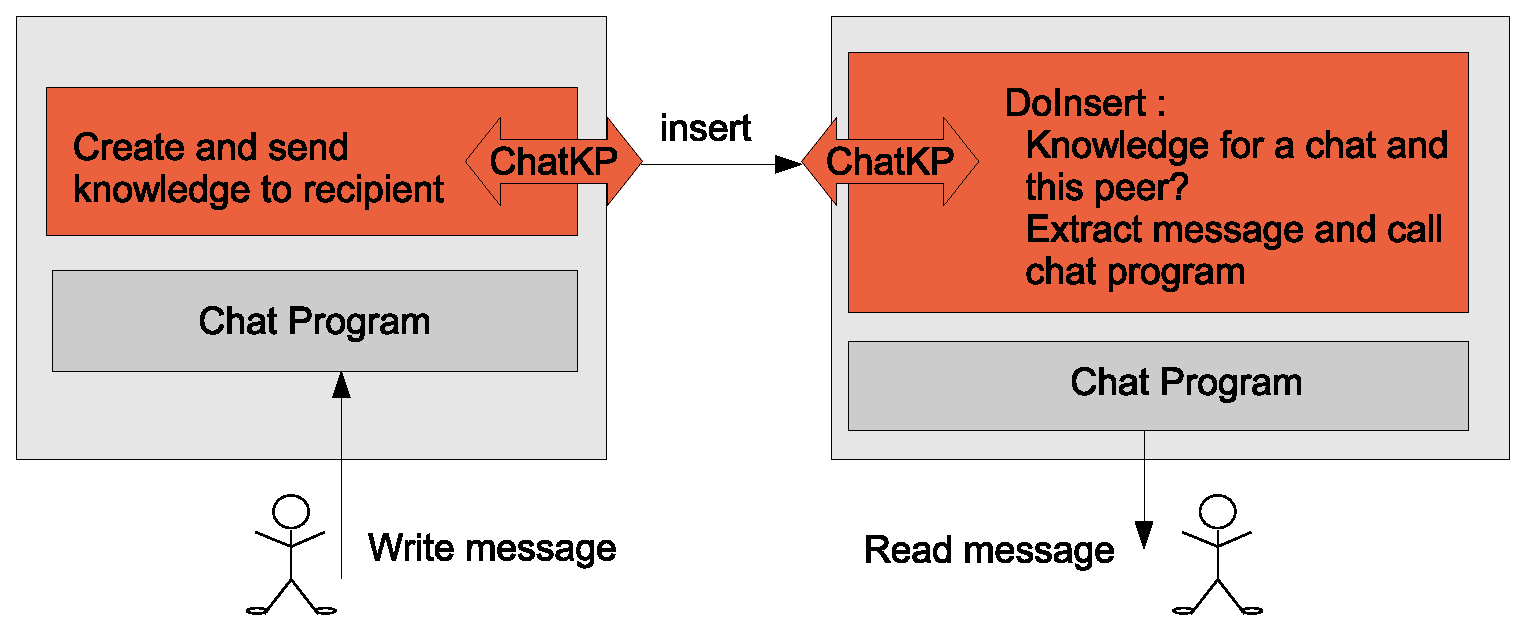
\includegraphics[width=0.90\textwidth]{chatKP.eps}
\caption{ChatKP - general idea}
\label{fig:chatKP}
\end{figure}

Figure \ref{fig:chatKP} illustrates (one possible) concept of a chat implementation with Shark. There is a user creating a message in the lower left corner. The message is written with a chat program. The message is transmitted to a {\tt ChatKP}. 

There are two data types in Shark which can be transmitted, interests and knowledge. The ''natural'' choice is wrapping the message into knowledge. Why is it ''natural''? A message is an arbitrary number of bytes. That is the definition of information in Shark. Information are transmitted inside knowledge. That's the reason.

{\tt ChatKP} creates knowledge which comprises several steps. First, a context point is created. It coordinates must be defined. In this implementation, the topic is set to a pre-defined semantic tag named {\it chat} and a unique subject identifier. Originator and peer is the creating peer. Remote peer is the recipient of that message. Multiple message are to be created for multiple recipients.

Knowledge is send to the recipient. A {\tt ChatKP} must be in place. It takes each incoming knowledge. It checks: Does this knowledge contain context point with a topic {\it chat}? Is it issued from an allowed peer? Is the receiving peer the intended recipient? If so, information from the context point can be extracted. The job of {\tt ChatKP} ends here. It isn't its job to interpret the message or interact with a user. It calls the local chat program to deal with the newly arrived message.

{\tt ChatKP} implementation is just a sketch but no ready for usage in a productive environment. There is no section {\it ChatKP usage} for that reason.

\subsection{Implementation}

\begin{figure}[t]
\centering
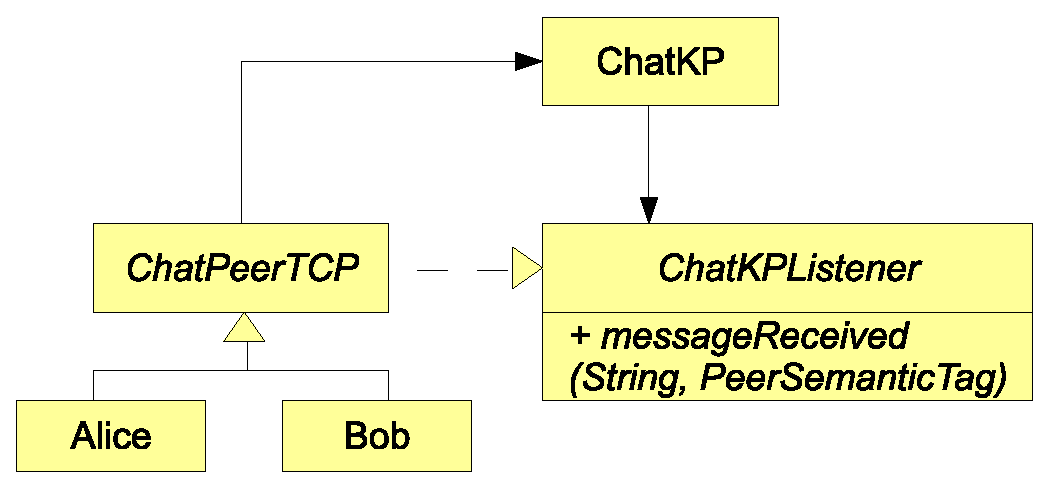
\includegraphics[width=0.70\textwidth]{chatClassDiagram.eps}
\caption{Chat implementation (sketch) - class diagram}
\label{fig:chatClassDiagram}
\end{figure}

Chat implementation is made up by four classes and one interface, see figure \ref{fig:chatClassDiagram}. {\tt ChatKPListener} is an interface that declares a single method: {\tt messageReceived}. This method is called by a {\tt ChatKP} whenever a new message arrived the peer. It has two parameter. First parameter is the actual message. Second parameter contains the sender. Later in this section we will have a look into {\tt ChatKP} implementation.

We have implemented an abstract class {\tt ChatPeerTCP}. It is abstract because is does {\it not} implement {\tt messageReceived}. Implementations are made in Alice and Bob. We start with Alice:

\subsection{Alice}

\begin{verbatim}
public class Alice extends ChatPeerTCP {

  public Alice(String peerName, String peerSI, 
               String address, int port) 
               throws SharkProtocolNotSupportedException, IOException {
    super(peerName, peerSI, address, port);
  }
\end{verbatim}

Alice extends {\tt ChatPeerTCP} which has a constructor that expects necessary data to describe a peer. Those data are: name of the peer, subject identifier, address and port. The final parameter already indicates: {\tt ChatPeerTCP} only uses TCP as protocol. As already noted - this program is a sketch but can be extended which is an exercise in this chapter. 

The main method brings no surprises:
\begin{verbatim}
  public static void main(String[] args) 
    throws SharkProtocolNotSupportedException, IOException {
    // setup alice peer
    Alice alice = new Alice("Alice", 
                            "http://www.sharksystem.net/alice.html",
                            "tcp://localhost:7070",
                            7070
     );

    System.out.println("Alice is running - start Bob now");
  }
}
\end{verbatim}

An object of class {\tt Alice} is created. Alice is described by the name ''Alice'' and her - now well-known - subject identifier. We use a local TCP address with port 7070. Note again: That program will run only on a single computer. It requires some (little) extensions to make it real chat.

Finally, we have a look at the {\tt messageReceived} implementation:
\begin{verbatim}
  @Override
  public void messageReceived(String message, PeerSemanticTag sender) 
                    throws SharkException, IOException {
    System.out.println("Alice has got that message:\n" + message);
    System.out.println("\nfrom:\n" + L.semanticTag2String(sender));
    System.out.println("Alice is going to reply with \"Hi Bob\"\n");
    this.chatKP.sendMessage("Hi Bob");

    // end of communication
    this.stop();
  }    
\end{verbatim}

The first three lines just print out the fact that a message was
received and from whom. Afterwords, a message (''Hi Bob'') is send
back. Apparently, a real chat program must prompt users entering
a reply. Finally, {\tt this.stop()} is called which is implemented in
{\tt ChatPeerTCP} and simply stops TCP communication in general. Thus, 
Alice sends a reply and shuts down whenever she receives a single message.
It is a sketch but illustrates the principle. The more interesting part are
implemented in {\tt ChatKP} anyway. But first have a look at the Bob implementation.

\subsection{Bob}
\begin{verbatim}

public class Bob extends ChatPeerTCP {

  public Bob(String peerName, String peerSI, String address, int port) 
             throws SharkProtocolNotSupportedException, IOException {
    super(peerName, peerSI, address, port);
  }
\end{verbatim}

The constructor is identical with Alice. It feeds the {\tt ChatPeerTCP} constructor.

\begin{verbatim}
  @Override
  public void messageReceived(String message, PeerSemanticTag sender) 
                              throws SharkException, IOException {
    System.out.println("Bob has received something:\n" + message);
    System.out.println("\nfrom:\n" + L.semanticTag2String(sender));

    // end of communication
    this.stop();
  }    
\end{verbatim}

Bob peer can receive a message. It is just printed out and communication is stopped. We already know Alice' behavior. She would send a message as soon as she has got one from Bob and terminate. Bob waits for a message and terminates without further actions.

\begin{verbatim}
  public static void main(String[] args) 
    throws SharkProtocolNotSupportedException, IOException, 
           SharkException, InterruptedException {

    System.out.println("Alice must run first");
    Bob bob = new Bob("Bob", 
                      "http://www.sharksystem.net/bob.html",
                      "tcp://localhost:7071",
                      7071
    );

    System.out.println("Bob started - send message to Alice");

    PeerSemanticTag alice = InMemoSharkKB.createInMemoPeerSemanticTag(
                            "Alice",                
                            "http://www.sharksystem.net/alice.html",
                            "tcp://localhost:7070");

    // send first message
    bob.chatKP.sendMessage("Hi Alice", alice);       
  } 
}
\end{verbatim}

A Bob object is created in main method. It uses port 7071. Bob creates a peer description for Alice which is required to call {\tt sendMessage()}. The final line asks {\tt chatKP} to send ''Hi Alice'' to the peer listening at port 7070 on localhost. 

The example works if the Alice program was started first. Alice would wait for incoming messages. Bob would send a message within its main method. Alice would get it, reply immediately and terminate. Bob would receive a reply print it out and stop working.

Let's have a look into {\tt ChatPeerTCP}.

\subsection{ChatPeerTCP}
\begin{verbatim}
public abstract class ChatPeerTCP implements ChatKPListener {
  private SharkEngine se = null;
  protected final ChatKP chatKP;
\end{verbatim}

That class implements a stand-alone program. It keeps a shark engine
and a {\tt ChatKP} as private member. Both are initialized in the
constructor we already know:

\begin{verbatim}
  public ChatPeerTCP(String peerName, String peerSI, 
                     String address, int port) 
                      throws SharkProtocolNotSupportedException, 
                             IOException {

    this.se = new J2SEAndroidSharkEngine();

    // create PeerSemanticTag describing peer itself
    PeerSemanticTag peer = InMemoSharkKB.createInMemoPeerSemanticTag
                           (peerName,    
                            peerSI, 
                            address);

    // create chat kp
    this.chatKP = new ChatKP(this.se, peer);

    // subscribe to news
    this.chatKP.addListener(this);

    // start listening at address - can throw exceptions
    this.se.startTCP(port);
  }
\end{verbatim}
We have already seen that Alice and Bob described themselves with
name, subject identifier and so forth. The constructor takes those parameters.
It creates a shark engine first. Second, a peer semantic tag is created that describes the peer itself (Alice or Bob in our example). Third, an object of
{\tt ChatKP} is created. It takes two parameters: Engine and peer that runs that
engine. Fourth, the objects subscribes to {\tt ChatKP} as listener. This call informs {\tt ChatKP} to call {\tt messageReceived} (implemented in Alice and 
Bob). Finally, the TCP connection is started. Now, the engine is listening at the defined port. It will receive incoming KEP message and transmit them to all active knowledge ports. In this program there is only one: {\tt ChatKP}.

\begin{verbatim}
  public void stop() {
    this.se.stop();
  }
}
\end{verbatim}
The final lines in this class implement the stop method. It is very simple. {\tt stop} in shark engine is called. The engine stops listening at any protocol. Open sessions remain unharmed, though.

\subsection{ChatKP}
Most work is done in {\tt ChatKP}. It can be re-used in productive programs.
We are going to skip some trivial parts of the program. The whole implementation can be found on Shark tutorials web page.

\begin{verbatim}
public class ChatKP extends KnowledgePort {
  public static final String CHAT_TOPIC_SI =
    "http://www.sharksystem.net/examples/chat/chatinterest.html";
  private PeerSemanticTag remotePeer = null;
  private ChatKPListener listener = null;
  private final PeerSemanticTag owner;

  public ChatKP(SharkEngine se, PeerSemanticTag owner) {
    super(se);
    this.owner = owner;
  }

  @Override
  protected void doExpose(SharkCS interest, KEPConnection kepConnection) {
  }
\end{verbatim}

{\tt ChatKP} is a {\tt KnowledgePort} and has to call its constructor
({\tt super(se);}). The engine object already exists and is transmitted as
parameter in its constructor. Some private member are declared. 
{\tt CHAT\_TOPIC\_SI} was defined as unique identifier for that chat implementation. It will be used in the topic dimension to create knowledge that can be send to another peer. {\tt remotePeer} will contain the peer with whom a chat will established. {\tt listener} will contain the chat program to which incoming messages are to be propagated. {\tt owner} is the peer that runs that chat.

That knowledge port does not handle interest. {\tt doExpose()} contains no action. That makes sense since whole message exchange is mapped on exchanging knowledge between peers.

Teh {\tt doInsert} makes the job:
\begin{verbatim}
  @Override
  protected void doInsert(Knowledge k, KEPConnection kepConnection) {
    Enumeration<ContextPoint> cpEnum = k.contextPoints();

    if(cpEnum != null) {
      ContextPoint cp = cpEnum.nextElement();
      ContextCoordinates cc = cp.getContextCoordinates();
      SemanticTag topic = cc.getTopic();
      if(!SharkCSAlgebra.identical(topic, this.getChatTopic())) {
        // this knowledge is not about chatting
        return;
      }

      PeerSemanticTag rPeer = cc.getRemotePeer();
      if(!SharkCSAlgebra.identical(rPeer, this.owner)) {
        // remote peer does not want to talk to me 
        return;
      }

      // remember that sender
      PeerSemanticTag peer = cc.getPeer();
      this.remotePeer = peer;

      // seems to be a chat message in knowledge - unwrap
      Iterator<Information> infoIter = cp.getInformation();
      if(infoIter != null) {
        String message;
        try {
          message = infoIter.next().getContentAsString();

          // notify listener about new message
          this.messageReceived(message, peer);
        } catch (Exception ex) {
        }
      }
    }
  }
\end{verbatim}

This method is called whenever knowledge reached that peer. First, it is tested if at least a single context point is present in the knowledge object. Second, it is tested if this context point is about ''chatting''. If not, the port aborts that algorithm. That knowledge has nothing to do with a chat.

Second, it is tested whether this peer is recipient of this chat message. Third, it is tested of the remote peer fits to accepted remote peers by this peer.

Information objects are extracted from the context point if all tests are passed. That message is transformed into a string an send to chat programs who have subscribed before. That's performed via {\tt this.messageReceived}.

Let's have look into this implementation:
\begin{verbatim}
  private void messageReceived(String message, PeerSemanticTag sender) 
                               throws SharkException, IOException {
    if(this.listener != null) {
      this.listener.messageReceived(message, sender);
    }
  }
\end{verbatim}

It's straightforward. A listener is called if a listener has be subscribed. We don't present subscribing implementation here. It is very simple.

Now, we have seen how {\tt ChatKP} handles incoming chat messages. Now we have to learn how it sends messages.

\begin{verbatim}

  public void sendMessage(String message, PeerSemanticTag recipient) 
                          throws SharkException, IOException {

    // first create coordinates
    SemanticTag chatTopic = this.getChatTopic();
    ContextCoordinates cc = InMemoSharkKB.createInMemoContextCoordinates(
                              chatTopic, // its a chat message
                              this.owner, // originator is owner of engine
                              this.owner, // peer is owner as well
                              recipient, // want to talk with connected peer
                              null, // time and place is irrelevant
                              null, 
                              SharkCS.DIRECTION_OUT
                             );

    // all metadata set - lets create a context point
    ContextPoint cp = InMemoSharkKB.createInMemoContextPoint(cc);

    // add message
    cp.addInformation(message);

    // create knowledge
    Knowledge k = InMemoSharkKB.createInMemoKnowledge();

    // add context point
    k.addContextPoint(cp);

    // send to remote peer
    this.sendKnowledge(k, recipient);
  }

  private SemanticTag getChatTopic() {
    SemanticTag chatTopic = InMemoSharkKB.createInMemoSemanticTag(
                              "ChatTopic",   
                               ChatKP.CHAT_TOPIC_SI);
    return chatTopic;
  }
}
\end{verbatim}

This message takes two parameter: message and recipient. This message has two wrap the message into a knowledge object. First, context coordinates are required. Seven parameter are required.

The topic is created with {\tt getChatTopic}. See also the method implementation. A semantic tag is created labeled with ''ChatTopic''. It semantics is defined by {\tt CHAT\_TOPIC\_SI}, see above. 

Originator and peer dimension is set to the owner of this engine. This makes
perfectly sense because this peer is creator and sender of the message. 

Remote peer is set to the recipient which is parameter of this method.

Location and time dimension remains empty. Spatial and temporal constraints are not necessary for this application.

Direction is set to {\tt OUT} because we are going to send something out.

A context point is created with those coordinates. The chat message can be attached as information. A knowledge object is created and the context point is added. Finally, that knowledge object is send out to the recipient peer with 
{\tt sendKnowledge(k, recipient)}.

The receiving peer would get a knowledge object via KEP-insert and call {\tt doInsert} on all active knowledge ports. We have already seen the {\tt ChatKP} implementation.

That's it. Download the chat program from our web page and let it run. Don't forget to run Alice first. Try to understand the program. Make it a real chat program afterwards, see also the exercises section in this chapter.

\section{Exercises}

\begin{enumerate}
\item 
Re-implement KP from last chapter but use {\tt StandardKP} as basis instead abstract class {\tt KnowledgePort}.
\item 
Extend {\tt ChatKP} to make it a real chat program.
\end{enumerate}
